\section{Markov Chains}\label{m:sec:markov-chains}

A Markov chain is specified by its state space and rules that determine future
states from the present one.  Its clock may advance in fixed steps or in continuous
time, a distinction that changes the analytical machinery without changing the
defining principle: conditional on the current state, the past supplies no further
information about the future.

\subsection{Discrete-Time Markov Chains}\label{m:sec:dtmc}

For a discrete-time chain $(X_n)_{n\geq0}$ on a countable state space
$\mathcal S$, the transition probabilities
\[
  P_{ij}=\pr{X_{n+1}=j\mid X_n=i}
\]
determine one-step evolution.  Repeated matrix multiplication gives multi-step
transition probabilities when the state space is conveniently enumerated; for
branching processes, generating-function composition is the more natural form of
the same iteration.

\subsubsection{Simple random walks}\label{m:sec:random-walks}

Simple random walks are intended to provide the elementary discrete-time example
and a first setting for hitting-probability problems.  The reviewed drafts, notes
and bibliography do not contain a substantive treatment, however, so this
subsection currently marks the source gap without supplying an unsourced transition
law, gambler's-ruin calculation or citation.  An approved treatment can be inserted
here without changing the surrounding architecture.

\subsubsection{Galton--Watson processes}\label{m:sec:gw}

The Galton--Watson process is a discrete-time Markov chain on the non-negative
integers.  If $Z_n$ is the size of generation $n$ and $L_1,L_2,\ldots$ are
independent copies of an offspring random variable $L$, then
\begin{equation}
  Z_{n+1}=\sum_{i=1}^{Z_n}L_i .
  \label{m:eq:gwrecursion}
\end{equation}
Writing $\phi(z)=\ex{z^L}$ and $\phi_n(z)=\ex{z^{Z_n}}$, independence gives
$\phi_{n+1}=\phi_n\circ\phi$.  Thus, if
$u_n=\pr{Z_n=0}$ for a process started from $Z_0=1$,
\begin{equation}
  u_{n+1}=\phi(u_n),\qquad u_0=0.
  \label{m:eq:gw-pgf-iteration}
\end{equation}

The binary law used throughout the thesis is
\begin{equation}
  \pr{L=2}=p,\qquad \pr{L=0}=1-p,
  \qquad \phi(z)=pz^2+1-p.
  \label{m:eq:binary-offspring}
\end{equation}
Its mean offspring number is $2p$, so
\begin{equation}
  \ex{Z_n}=(2p)^n.
  \label{m:eq:meanZn}
\end{equation}
With $S_n=\pr{Z_n>0}=1-u_n$, \cref{m:eq:gw-pgf-iteration} becomes
\begin{equation}
  S_{n+1}=2pS_n-pS_n^2,\qquad S_0=1.
  \label{m:eq:SnIter}
\end{equation}
The present framework needs only this definition, its one-step structure and the
survival recursion.  Two consequences are nevertheless worth recording.  At the
critical value $p=\tfrac12$,
\begin{equation}
  S_n\sim\frac{2}{n},
  \qquad
  \pr{T=n+1}\sim\frac{2}{n^2},
  \label{m:eq:critical-summary}
\end{equation}
where $T=\inf\{n:Z_n=0\}$, while the total progeny
$\mathcal T=\sum_{n\geq0}Z_n$ obeys an exact Catalan law and has a
$k^{-3/2}$ mass-function tail.  The short reciprocal-increment proof and the
tree count are collected in \cref{m:app:critical-gw}.  Discrete functional
iteration returns briefly in \cref{m:sec:discrete-methods}, before \ChA{}
develops the fuller Koenigs-function treatment of the constant $A(p)$.

\begin{figure}[H]
  \centering
  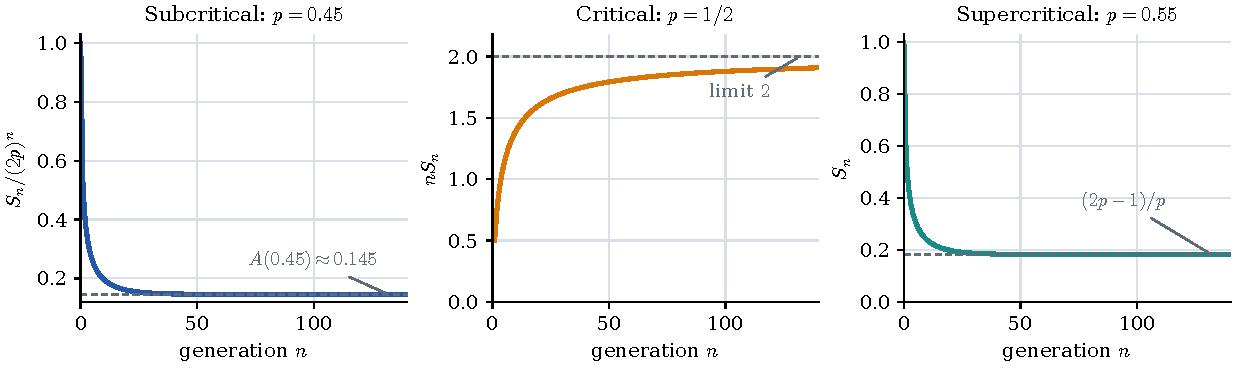
\includegraphics[width=\textwidth]{figures/generated/gw_regime_diagnostics.pdf}
  \caption{Three regime-specific diagnostics for the binary survival recursion
  \cref{m:eq:SnIter}.  In the subcritical case, removal of the geometric factor
  reveals the amplitude $A(p)$; at criticality, $nS_n$ approaches $2$; and in the
  supercritical case, survival approaches the positive fixed point
  $(2p-1)/p$.  Each curve is obtained by direct iteration from $S_0=1$.}
  \label{m:fig:gw-regime-diagnostics}
\end{figure}

\subsubsection{Founding bottlenecks and conditioned histories}
\label{m:sec:founding-bottlenecks}

Asymptotic criticality does not remove the early bottleneck faced by a small
founding population.  At $p=\tfrac12$, the first four extinction probabilities
are
\[
  u_1=0.500,\qquad u_2=0.625,\qquad
  u_3=0.6953125,\qquad u_4=0.7417297\ldots.
\]
For $k$ independent founders, all $k$ descendant trees are extinct by generation
$n$ with probability $u_n^k$, and hence
\begin{equation}
  S_n^{(k)}=1-u_n^k=1-(1-S_n)^k.
  \label{m:eq:k-founder-survival}
\end{equation}
This identity separates the one-lineage dynamics from the effect of the founding
size.  It also makes the relevant selection effect visible: conditioning an
ensemble on late survival enriches it for paths with unusually favourable early
growth, even though every path was generated by the same offspring law.  This
``push of the past'' is a survivorship effect rather than a change in mechanism
\cite{Budd2018}.  The early-generation calculation, cohort comparison and its
interpretation are developed in \cref{m:app:small-populations}.

\subsubsection{A discrete rupture bridge}
\label{m:sec:discrete-rupture-bridge}

The same pathwise viewpoint supplies a discrete precursor of catastrophe.  If
each individual initiates rupture independently with probability $\kappa$ per
generation, and $H_n=\sum_{i=0}^{n-1}\widetilde Z_i$ is the accumulated exposure
of the catastrophe-free genealogy, then
\begin{equation}
  \pr{\text{no rupture before }n}
  =\ex{(1-\kappa)^{H_n}}
  \geq (1-\kappa)^{\ex{H_n}}.
  \label{m:eq:rupture-jensen-summary}
\end{equation}
The inequality is Jensen's, not a mean-field identity.  In particular, it bounds
non-rupture and does not by itself bound the joint event of non-rupture and
population survival.  The deterministic doubling calculation and the exact
random-exposure formula appear in \cref{m:app:discrete-rupture}.

\subsection{Continuous-Time Markov Chains}\label{m:sec:ctmc}

Let $(X_t)_{t\geq0}$ take values in a countable state space $\mathcal S$.  A
time-homogeneous continuous-time Markov chain is specified by its generator
$Q=(q_{ij})$, where
\begin{equation}
  q_{ij}=\lim_{h\downarrow0}\frac{\pr{X_{t+h}=j\mid X_t=i}}{h}
  \quad(j\neq i),\qquad
  q_{ii}=-\sum_{j\neq i}q_{ij}=:-q_i.
  \label{m:eq:generator}
\end{equation}
The holding time in state $i$ is exponential with rate $q_i$, after which the
chain jumps to $j$ with probability $q_{ij}/q_i$.  An exponential random variable
$T$ of rate $\theta$ has
\[
  \pr{T>t}=\ee^{-\theta t},\qquad \ex{T}=\theta^{-1},
\]
and is memoryless.  If independent clocks of rates $\theta_1,\ldots,\theta_m$
compete, their minimum has rate $\Theta=\sum_i\theta_i$ and clock $k$ wins with
probability
\begin{equation}
  \pr{T_k=\min_iT_i}=\frac{\theta_k}{\Theta}.
  \label{m:eq:competing-clocks}
\end{equation}
This rate-to-probability conversion supplies the interface between discrete and
continuous birth--death descriptions and underlies direct trajectory simulation
\cite{Gillespie1977}.

If $P(t)=(p_{ij}(t))$ is the transition matrix, the forward Kolmogorov equation is
\begin{equation}
  \frac{\dd P}{\dd t}=P Q.
  \label{m:eq:kolmogorov-forward}
\end{equation}
For a fixed initial distribution, its component form is the master equation
\begin{equation}
  \ddt{p_j(t)}=\sum_{k\neq j}q_{kj}p_k(t)-q_jp_j(t).
  \label{m:eq:master}
\end{equation}
The first term collects probability entering $j$, whereas the second records all
probability leaving it.

\subsubsection{Poisson processes}\label{m:sec:poisson}

A Poisson-process introduction is intended to precede the general birth--death
examples.  The reviewed sources support the exponential holding-time and competing-
clock machinery above, but provide no substantive construction, counting law or
citation for the associated counting process.  This subsection therefore records
that source boundary and awaits an approved account; no further axioms or formulae
are introduced here.

\subsubsection{Birth--death processes}\label{m:sec:birth-death}

In the linear birth--death process, each of the $n$ individuals present contributes
independently to birth and death.  The non-zero rates from state $n$ are
\begin{equation}
  q_{n,n+1}=\lambda n,\qquad q_{n,n-1}=\mu n,
  \label{m:eq:bdrates}
\end{equation}
and $0$ is absorbing.  The state probabilities satisfy
\begin{equation}
  \ddt{p_n}=\lambda(n-1)p_{n-1}+\mu(n+1)p_{n+1}
  -(\lambda+\mu)n p_n.
  \label{m:eq:bdmaster}
\end{equation}
Equivalently, the generator acts on a test function $f$ by
\begin{equation}
  (\mathcal Lf)(n)
  =\lambda n\{f(n+1)-f(n)\}
   +\mu n\{f(n-1)-f(n)\}.
  \label{m:eq:bd-generator-action}
\end{equation}
Choosing an indicator function recovers one column of the master equation, while
choosing a power or falling factorial produces a moment equation.  These uses are
developed in \cref{m:sec:continuous-methods}.

The rates also give a direct pathwise construction.  Conditional on $X_t=n>0$,
the next event time is exponential with parameter $n(\lambda+\mu)$.  Over a short
interval $h$,
\begin{align}
  \pr{X_{t+h}=n+1\mid X_t=n}&=\lambda n h+o(h),\notag\\
  \pr{X_{t+h}=n-1\mid X_t=n}&=\mu n h+o(h),\notag\\
  \pr{X_{t+h}=n\mid X_t=n}&=1-n(\lambda+\mu)h+o(h).
  \label{m:eq:bd-infinitesimal-transitions}
\end{align}
These relations determine both the jump chain and its clock.  They also explain
why the model has two complementary descriptions.  At population level it is a
nearest-neighbour chain with state-dependent speed; at individual level it is the
sum of independent descendant families, each begun by one founder.

Let $X_t^{(r)}$ denote the descendants at time $t$ of founder $r$.  Starting from
$N$ individuals,
\begin{equation}
  X_t=\sum_{r=1}^{N}X_t^{(r)},
  \qquad
  X_t^{(1)},\ldots,X_t^{(N)}\ \hbox{independent and identically distributed}.
  \label{m:eq:bd-family-decomposition}
\end{equation}
This decomposition is stronger than a statement about means.  If
$F(z,t)=\ex{z^{X_t}\mid X_0=1}$, then
\begin{equation}
  \ex{z^{X_t}\mid X_0=N}=F(z,t)^N.
  \label{m:eq:bd-branching-property}
\end{equation}
Thus the law for every fixed initial population is determined by the one-founder
law.  Extinction by time $t$ is the specialisation $z=0$, so its probability from
$N$ founders is the $N$th power of the one-founder probability.  Differentiation
at $z=1$ instead shows that the mean is $N$ times the one-founder mean.  These are
two consequences of the same factorisation, not separate assumptions.

\begin{figure}[tbp]
  \centering
  \begin{tikzpicture}[
    font=\small,
    state/.style={circle, draw=blue!60!black, fill=blue!7,
      minimum size=9.5mm, inner sep=1pt},
    zero/.style={circle, double, draw=gray!70!black, fill=gray!8,
      minimum size=10mm, inner sep=1pt},
    jump/.style={-{Stealth[length=2.1mm]}, semithick, draw=gray!75!black}
  ]
    \node[zero] (zero) {$0$};
    \node[state, right=18mm of zero] (one) {$1$};
    \node[state, right=22mm of one] (two) {$2$};
    \node[state, right=22mm of two] (three) {$3$};
    \node[right=16mm of three] (dots) {$\cdots$};
    \draw[jump, bend left=17] (one) to node[above] {$\lambda$} (two);
    \draw[jump, bend left=17] (two) to node[below] {$2\mu$} (one);
    \draw[jump, bend left=17] (two) to node[above] {$2\lambda$} (three);
    \draw[jump, bend left=17] (three) to node[below] {$3\mu$} (two);
    \draw[jump] (one) -- node[above] {$\mu$} (zero);
    \draw[jump] (three) -- node[above] {$3\lambda$} (dots);
  \end{tikzpicture}
  \caption{The linear birth--death chain.  Per-individual rates make both the
  total event rate and the speed of the clock proportional to the current
  population; state $0$ is absorbing.}
  \label{m:fig:birth-death-chain}
\end{figure}
The total event rate in state $n$ is $n(\lambda+\mu)$, so the holding time has
mean $\{n(\lambda+\mu)\}^{-1}$.  Conditional on a jump, its direction is
independent of $n$:
\begin{equation}
  \pr{n\to n+1\mid\text{a jump}}=\frac{\lambda}{\lambda+\mu},
  \qquad
  \pr{n\to n-1\mid\text{a jump}}=\frac{\mu}{\lambda+\mu}.
  \label{m:eq:bd-embedded-chain}
\end{equation}
Thus the embedded jump chain records the relative rates, while the continuous
clock accelerates as the population grows.  The independence of descendant
families also gives a branching property: if $F(z,t)$ is the PGF from one founder,
then the PGF from $N$ founders is $F(z,t)^N$.

The embedded chain alone cannot answer time-dependent questions.  For example,
two processes with rates $(\lambda,\mu)$ and $(c\lambda,c\mu)$ have the same jump
directions but different holding times: multiplying both rates by $c$ accelerates
the continuous trajectory by the same factor.  Conversely, changing the ratio
$\lambda/\mu$ changes the drift of the event sequence itself.  This separation is
useful in simulation and analysis.  One first samples a wait of rate
$n(\lambda+\mu)$ and then samples the jump direction using
\cref{m:eq:bd-embedded-chain}; analytically, first-step equations perform exactly
the same two-stage conditioning.

For the probability generating function
$G(z,t)=\sum_{n\geq0}p_n(t)z^n$, index shifts turn this infinite system into
\begin{equation}
  \pddt{G}=(\lambda z-\mu)(z-1)\pdd{G}{z},
  \qquad G(z,0)=z^N.
  \label{m:eq:bdpde}
\end{equation}
To see where the polynomial coefficient comes from, multiply
\cref{m:eq:bdmaster} by $z^n$ and sum over $n\geq0$.  The birth inflow, death
inflow and total outflow become, respectively,
\begin{equation}
  \lambda z^2G_z,
  \qquad \mu G_z,
  \qquad-(\lambda+\mu)zG_z.
  \label{m:eq:bd-index-shifts}
\end{equation}
Their sum factorises as $(\lambda z-\mu)(z-1)G_z$.  The root $z=1$ expresses
conservation of total probability, since \cref{m:eq:bdpde} then gives
$\partial_tG(1,t)=0$.  The other root, $z=\mu/\lambda$, encodes the extinction
threshold and reappears in the characteristic solution.

The PGF retains the full state law.  At any fixed time,
\begin{equation}
  p_n(t)=\frac{1}{n!}\left.\frac{\partial^nG}{\partial z^n}\right|_{z=0},
  \qquad
  p_0(t)=G(0,t),
  \qquad
  \ex{X_t}=G_z(1,t).
  \label{m:eq:bd-pgf-recovery}
\end{equation}
The points $z=0$ and $z=1$ therefore answer different questions: the first
extracts absorption at zero, while derivatives at the second extract moments of
the unabsorbed distribution.  The characteristic solution in
\cref{m:sec:extinction-probabilities} makes both evaluations explicit.
This process becomes the main example in \cref{m:sec:continuous-methods}, where the
same equation yields moments, extinction probabilities and conditional means.

\subsubsection{Birth--death--catastrophe processes}\label{m:sec:bdc}

A birth--death--catastrophe chain adds an abrupt transition to a distinct absorbing
state $\dagger$.  For the linear version used later, the rates from $n\geq1$ are
\begin{equation}
  q_{n,n+1}=\lambda n,\qquad
  q_{n,n-1}=\mu n,\qquad
  q_{n,\dagger}=\rho n,
    \label{m:eq:bdcrates}
\end{equation}
with both $0$ and $\dagger$ absorbing.  The two absorbing mechanisms are not
interchangeable.  Ordinary extinction reaches $0$ through successive deaths,
whereas catastrophe removes the current population in one event.  On the
non-catastrophe states, the sub-probability generating function
\[
  G(z,t)=\ex{z^{X_t}\mathbf 1\{X_t\neq\dagger\}}
\]
satisfies
\begin{equation}
  \pddt{G}=
  \bigl(\lambda z^2-(\lambda+\mu+\rho)z+\mu\bigr)\pdd{G}{z},
  \qquad G(z,0)=z^N.
  \label{m:eq:bdcpde}
\end{equation}
Unlike \cref{m:eq:bdpde}, this PDE need not conserve $G(1,t)$, because its missing
mass is precisely the probability already removed by catastrophe.  A
population-dependent catastrophe rate also reweights whole paths through their
accumulated exposure and therefore cannot be replaced by a hazard evaluated at the
mean population.

\begin{figure}[tbp]
  \centering
  \begin{tikzpicture}[
    font=\small,
    state/.style={circle, draw=blue!60!black, fill=blue!7,
      minimum size=10mm, inner sep=1pt},
    absorb/.style={circle, draw=red!65!black, fill=red!8,
      minimum size=11mm, inner sep=1pt, double},
    jump/.style={-{Stealth[length=2.2mm]}, semithick, draw=gray!75!black},
    kill/.style={-{Stealth[length=2.2mm]}, semithick, draw=red!70!black}
  ]
    \node[state] (minus) {$n-1$};
    \node[state, right=30mm of minus] (centre) {$n$};
    \node[state, right=30mm of centre] (plus) {$n+1$};
    \node[absorb, below=21mm of centre] (dagger) {$\dagger$};

    \draw[jump, bend left=16] (centre) to node[above] {$\lambda n$} (plus);
    \draw[jump, bend left=16] (plus) to node[below] {$\mu(n+1)$} (centre);
    \draw[jump, bend left=16] (centre) to node[below=2pt] {$\mu n$} (minus);
    \draw[jump, bend left=16] (minus) to node[above=2pt] {$\lambda(n-1)$} (centre);
    \draw[kill] (centre) -- node[right] {$\rho n$} (dagger);
  \end{tikzpicture}
  \caption{Local transition structure of the linear
  birth--death--catastrophe chain.  The horizontal birth and death moves repeat
  on the non-negative integers; $0$ and the catastrophe state $\dagger$ are
  absorbing.}
  \label{m:fig:bdc-transitions}
\end{figure}

Restricting the generator to the positive states makes the absorption mechanism
especially clear.  For general birth, death and catastrophe rates
$\lambda_i,\mu_i,\kappa_i$, the killed subgenerator $K$ has
\begin{equation}
  K_{i,i+1}=\lambda_i,\qquad
  K_{i,i-1}=\mu_i\ (i\geq2),\qquad
  K_{i,i}=-(\lambda_i+\mu_i+\kappa_i).
  \label{m:eq:bdc-subgenerator}
\end{equation}
The missing row mass is the instantaneous absorption rate.  If $T$ is the time
of either ordinary extinction or catastrophe, summing the positive-state forward
equations gives
\begin{equation}
  \frac{\dd}{\dd t}\pr{T>t}
  =-\mu_1\pr{X_t=1}-\sum_{i\geq1}\kappa_i\pr{X_t=i},
  \label{m:eq:bdc-survival-loss}
\end{equation}
where the probabilities refer to the chain before absorption.  Ordinary death
removes survival mass only from state $1$; catastrophe may remove it from every
positive state.

If $\nu$ is quasi-stationary for the killed chain, then for some $\theta>0$
\begin{equation}
  \nu K=-\theta\nu,
  \qquad
  \mathbb P_{\nu}(T>t)=\ee^{-\theta t},
  \qquad
  \theta=\mu_1\nu_1+\sum_{i\geq1}\kappa_i\nu_i.
  \label{m:eq:bdc-qsd-eigenrelation}
\end{equation}
A constant catastrophe clock merely shifts the survival decay rate and leaves the
law conditional on survival unchanged.  State-dependent catastrophe instead
reweights paths by their accumulated exposure, precisely the distinction already
visible in \cref{m:eq:rupture-jensen-summary}.

\subsection{Time-Inhomogeneous Processes}\label{m:sec:time-inhomogeneous}

Time-inhomogeneous chains allow their transition rules to depend explicitly on
calendar time.  The intended thesis example is a logistic speciation model, but the
reviewed sources contain no equations, parameter definitions or citations from
which that model can be reconstructed.  The subsection therefore remains an
explicit source-gap marker until author-approved material supplies its state space,
time-dependent rates and logistic mechanism.

\subsection{Coupled ODE--CTMC Systems}\label{m:sec:coupled-ode-ctmc}

The final process class couples deterministic continuous variables to a
continuous-time Markov chain.  The ODE dynamics may depend on the chain state, the
chain's transition rates may depend on the ODE variables, or the dependence may
operate in both directions.  The reviewed sources contain no concrete coupled
model, governing ODE, rate functions or citation, so this subsection records only
the intended interface.  Its mathematical development awaits author-approved
source material rather than an invented schematic example.
